\title{\LARGE \bf
Assessment of Nine Large Market Capitalization Securities\\
\large
STAT4290 Final Project }
\author{Patrick Rogan, Qitong Liu, Shuni Fang, Xuyan Xiao}

\documentclass[10pt]{article_simple}
\usepackage[utf8]{inputenc}
\usepackage{tabularx}
\usepackage[margin=.85in]{geometry}
\usepackage{amssymb}
\usepackage{amsmath}
\usepackage{graphicx}
\usepackage{caption}
\usepackage{subcaption}
\usepackage{float}
\usepackage{framed}

\newpage
\setcounter{page}{1}
\renewcommand{\thepage}{Rogan $\cdot$ Qitong $\cdot$ Fang $\cdot$ Xiao - \arabic{page}}

\newcolumntype{P}[1]{>{\centering\arraybackslash}m{#1}}

\begin{document}
\maketitle

\begin{abstract}
Nine publicly traded companies were selected from from the largest holdings of Berkshire Hathaway as of September 30, 2015 [1]. Five year asset and T-Bill returns from the United States Federal Reserve Bank were examined and combined into portfolios that were assessed on the basis of annualized returns, risk and monthly Value at Risk (VaR) and Expected Shortfall (ES) [2]. A time series analysis was performed on the S\&P 500 in order to provide an outlook for the assets and portfolios examined. Portfolios generated from the assets selected have high annualized returns ($7\% < R < 21\%$) and can be constructed in a manner to substantially limit risk. Time series analysis of the S\&P 500 suggests a positive outcome for short term investment while additional caution is required for longer term investment decisions.
\end{abstract}

\section*{Asset Analysis}

Monthly price and return data (adjusted for splits and dividends) were analyzed for nine assets. Company characteristics are summarized and univariate distributions fit to individual asset returns, see Table 1.

\vspace{1em}

\begin{small}
\begin{minipage}{\linewidth}
\begin{center}
\begin{tabular}{ |P{3.5cm}||P{1.7cm}|P{1.7cm}|P{1.7cm}|P{1.7cm}|P{1.8cm}|  }
 \hline
 \multicolumn{6}{|c|}{\textbf{	Asset Summary}} \\
 \hline
 Company  &  Ticker Symbol & Sector &  Market Capitalization  &  $\beta$ & Best Fit Distribution \\
 \hline
American Express &AXP& 	Services & 69.4B & 0.91 & t \\
 \hline
International Business Machine &IBM&Technology & 135.4B & 0.59 & ged\\
 \hline
Coca-Cola &KO& Consumer Goods & 187.7B &  0.49 & skewed ged\\
 \hline
Moody's Corporation &MCO& Services & 20.6B &1.23 & ged\\
 \hline
Wells Fargo \& Company &WFC& Financial & 282.7B & 0.94 & ged\\
 \hline
DaVita HealthCare Partners &DVA&Healthcare & 15.1B &  0.99 & t\\
 \hline
Procter \& Gamble Company &PG& Consumer Goods & 212.7B &  0.57 & ged\\
 \hline
U.S. Bancorp &USB&Financial &76.9B &  0.79 & skewed t\\
 \hline
Wal-Mart Stores &WMT&	Services & 193.4B & 0.27 & t\\
 \hline
\end{tabular}
\bigskip \\
Table 1. Summary of nine large market capitalization assets. Several sectors are represented. Best fitted distribution was determined by AIC.
\end{center}
\end{minipage}
\end{small}

General statistics were calculated for all assets, see Appendix A, Figure 7. Average monthly returns for all assets were found to range between 0.0 and 0.03. Additionally, the monthly returns of each of the nine assets were found to fluctuate around 0. Augmented Dickey-Fuller Tests were run on all assets and all returns were found to be stationary.

Monthly asset prices were examined and equity curves were generated, see Figure 1. Approximately half of the assets outperform the S\&P 500 during this time interval, see Appendix A, Figure 6. There are clear upward trends in the prices of KO and DVA, MCO, WFC, and USB. Notice that WMT has a gradual price drop starting throughout 2015 and IBM has been trending downward since 2013. We believe that the price drop in WMT  is caused by two main reasons. One is the announcement that it planned to hike the minimum wage for its U.S. workforce, which would cost an additional \$1.2 billion in 2015 and \$1.5 billion in 2016. The other reason is that as Wal-Mart continues to invest in online grocery service, which shows the potential for massive growth, the upfront cost remains an issue for investors. For IBM, the stock appears to have been oversold since the summer of 2013, which leads to the downward trend of the stock price.

\begin{figure}[H]
	\centering
  	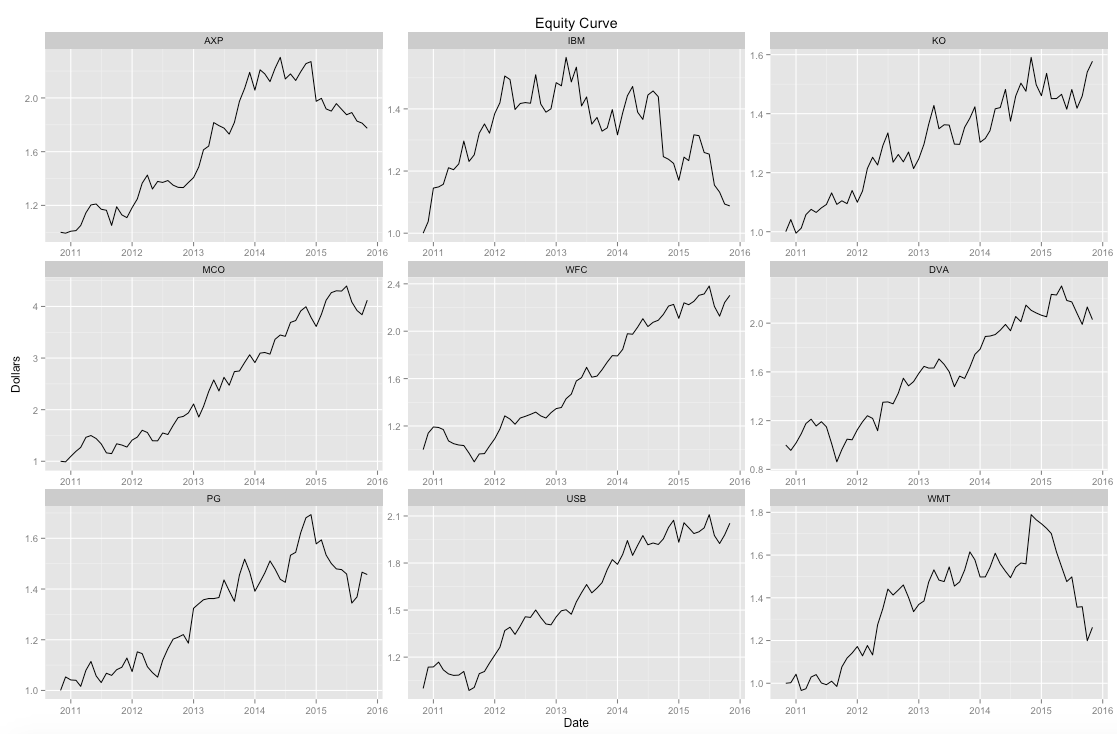
\includegraphics[width=.75\linewidth]{equity_curve_adjusted}
  	\centering
  	\caption{Equity curves for all assets examined.}
\end{figure}

Principle component analysis (PCA) was performed on the returns of assets, see Figure 2. All assets have negative correlation with the first principal component (PC1) indicating a positive movement would result in losses for all stocks. However, it is also noted that the the the correlation between assets and the remaining PCs is much more varied. Also note the first PC accounts for 42.4\% of the total variance and 8 of 9 PCs are required to account for $>95\%$ of the total variance, see Appendix A, Figure 14. The data suggest diverse portfolios can be constructed from these assets.

\begin{figure}[H]
	\centering
	\begin{subfigure}{.45\textwidth}
  	\centering
  	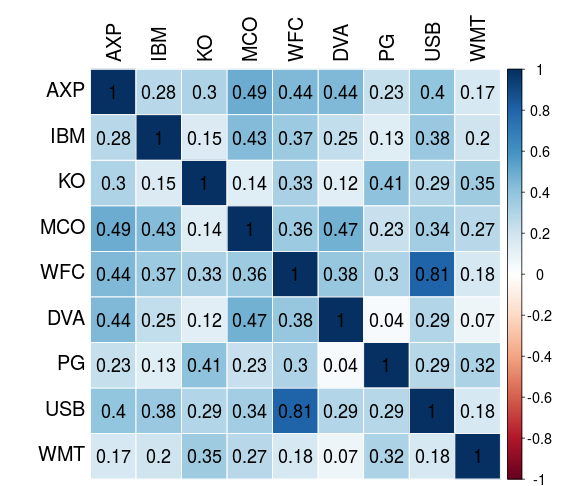
\includegraphics[width=.9\linewidth]{Correlation_Matrix}
  	\caption{Correlation matrix of asset returns, note all correlations are positive.}
    \label{fig:sub1}
	\end{subfigure}%
		\hspace{1em}
	\begin{subfigure}{.45\textwidth}
  	\centering
  	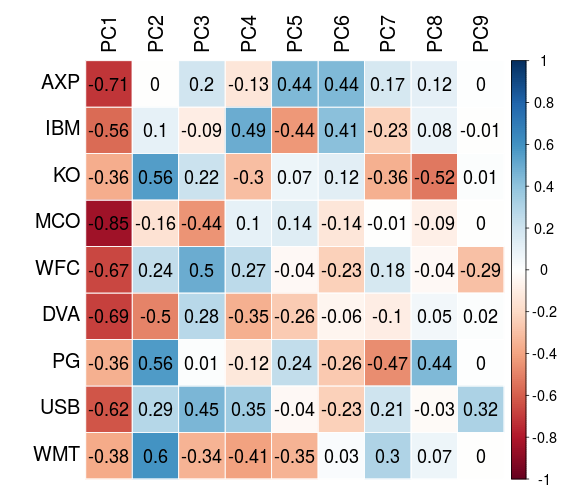
\includegraphics[width=.9\linewidth]{Correlation_Matrix_top_Right}
  	\caption{Correlation of assets returns with asset return principal components}
 	\label{fig:sub2}
	\end{subfigure}
	\caption{Asset and PC correlations, note for PCA analysis some companies within the same sector appear to have similar relations to first and second principle components, for example KO and PG or WFC and UBS where as other companies in the same sectors do not ie APX, WM and MC.}
\end{figure}

\section*{Portfolio Analysis}
In order to determine an optimal investment strategy, six portfolios were constructed from the nine companies and risk free asset determined from the monthly T-Bill returns: Minimum Variance Portfolios without/with Short Selling allowed, Tangency Portfolios without/with Short selling Allowed, and Two Portfolios with a targeted annual return of 12\%, see Figure 3.

The portfolios were constructed in such a manner that their asset allocation was unconstrained except for the case of the portfolios with shorting allowed. Here asset weights were constrained to $-10\% < w_i < 80\%$ to prevent potentially risky large short positions. However, some portfolios still had unbalanced asset allocations relying heavily on companies in the finance/financial services sectors, see Appendix B, Table 9.

\begin{figure}[H]
\centering
	\begin{subfigure}{.45\textwidth}
  	\centering
  	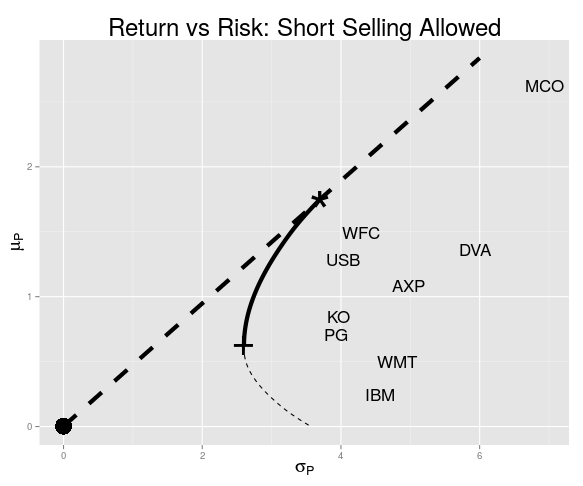
\includegraphics[width=.95\linewidth]{Tangency}
  	\caption{Short selling allowed with individual assets weights constrained to $-10\% < w_i < 80\%$.}
    \label{fig2:sub1}
	\end{subfigure}%
	\hspace{1em}
	\begin{subfigure}{.45\textwidth}
  	\centering
  	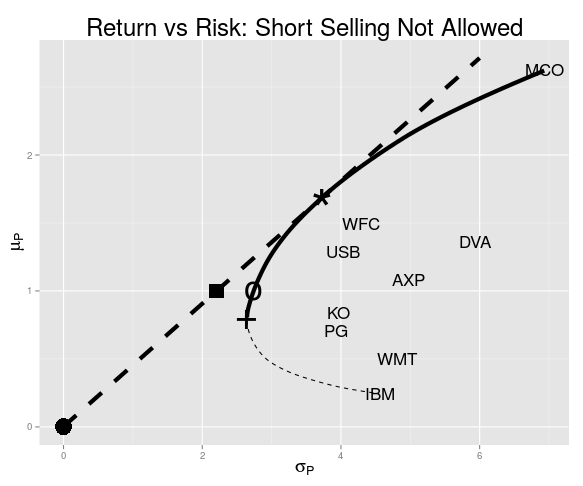
\includegraphics[width=.95\linewidth]{Tangency_NOS}
  	\caption{Portfolio with short selling disallowed. No constraints imposed on asset weights.}
 	\label{fig2:sub2}
	\end{subfigure}
	\caption{Efficient Fronter (Solid Line), Line of Efficient Portfolios (Heavy Dashed Line), Inefficient Portfolios (Light Dashed Line), Minimum Variance Portfolio (+), Risk Free ($\cdot$), Tangency Portfolio (*), Efficient Portfolio with 1.0\% Monthly Return (o), Combination Tangency and Risk Free with 1.0\% Monthly Return ($\blacksquare$).}
\end{figure}
Portfolio viability was assessed on the basis of expected annualized risk and return along with copula-based portfolio VaR assessments. Annualized portfolio characteristics were generated for the Minimum Variance Portfolios without/with Short Selling allowed and Tangency Portfolios without/with Short selling Allowed, see Table 2.

\begin{small}
\vspace{1em}
\begin{minipage}{\linewidth}
\begin{center}
\begin{tabular}{ |P{2.2cm}||P{2.2cm}|P{2.2cm}|P{2.2cm}|P{2.2cm}|  }
 \hline
 \multicolumn{5}{|c|}{\textbf{Portfolio Characteristics (Annualized)}} \\
 \hline
   &  Min Variance  (No Shorts) &  Min Variance &   Tangency (No Shorts)  &    Tangency  \\
 \hline
Return  &      9.53&  7.49& 20.27&  21.00\\
Risk   &       9.16&  9.01&  9.67&  12.81\\
$\sigma^2$ &     83.97& 81.23& 93.45& 164.08\\
Sharpe Ratio&  1.04&  0.83&  2.09&   1.64\\
 \hline
\end{tabular}
\bigskip \\
Table 2. Measures of portfolio risk and return. Note the minimum variance portfolios have Sharpe ratios similar to the individual assets while tangency portfolios have higher Sharpe ratios than any individual asset.
\end{center}
\end{minipage}
\end{small}

The two tangency portfolios have higher expected returns than the minimum variance portfolios while only having higher variances than the observed minimum values. The tangency portfolio with short selling has only a slightly higher return than that of the tangency portfolio that does not allow for shorting. As there is significantly more risk in the tangency portfolio that allows for shorting, the slightly higher return does not justify potential investment.

To further quantify risk, individual asset monthly ES and VaR values were obtained and confidence intervals were established for both parametric and nonparametric bootstraps, see Appendix B, Table II. While these values provide approximate bounds to potential losses, a higher fidelity measure of risk was computed using a t-copula, see Appendix C. 5\% VaR and ES monthly estimates were computed for all portfolios, see Tables 3 and 4.

\begin{small}
\vspace{1em}
\begin{minipage}{\linewidth}
\begin{center}
\begin{tabular}{ |P{2.2cm}||P{2.2cm}|P{2.2cm}|P{2.2cm}|P{2.2cm}|  }
 \hline
 \multicolumn{5}{|c|}{\textbf{Monthly VaR and ES by Portfolio}} \\
 \hline
   &  Min Variance  (No Shorts) &  Min Variance &   Tangency (No Shorts)  &    Tangency  \\
 \hline
$\widehat{VaR}^t(0.05)$ & 3537 & 3635 & 2879 & 4303  \\
$\widehat{ES}^t(0.05)$ & 4773 & 4851 & 4183 & 6031 \\
  \hline
\end{tabular}
\bigskip \\
Table 3. Monthly VaR and ES estimates assuming \$100,000.00 invested in each portfolio.
\end{center}
\end{minipage}
\end{small}

\begin{small}
\vspace{1em}
\begin{minipage}{\linewidth}
\begin{center}
\begin{tabular}{ |P{2.2cm}||P{2.2cm}|P{2.2cm}|  }
 \hline
 \multicolumn{3}{|c|}{\textbf{Monthly Risk for 12\%/year Return Portfolios}} \\
 \hline
   &  Efficient Portfolio &  Tangency w/ Risk Free \\
 \hline
Risk&   2.74& 2.21\\
$\widehat{VaR}^t(0.05)$& 3484 & 1545  \\
$\widehat{ES}^t(0.05)$ &  4764 & 2155 \\
 \hline
\end{tabular}
\bigskip \\
Table 4. Risk metrics for portfolios with 12\% targeted annualized return; VaR and ES are calculated for a portfolio of \$100,000.00. Note the tangency portfolio with risk free asset achieves a moderate return with extremely low VaR and ES values.
\end{center}
\end{minipage}
\end{small}

Generally, VaR and ES values for portfolios were smaller than for individual assets given equivalent investment. Given all measures of risk and return, several of the derived portfolios would likely be attractive for investors depending on individual objectives.

\section*{Time Series Analysis on S\&P500}

A straightforward investment strategy is to invest in an index fund. Accordingly, a time series analysis was performed on the S\&P500 index. This analysis gives an expected investment outcome based on past market performance,  see Appendix D, Figure 18. Given all assets used in the generation of portfolios have positive correlations with the S\&P 500, this estimate of future returns can be used to determine when market conditions are favorable.

\subsection*{Stationariness}
Autocorrelation Function (ACF) plots of the returns and the prices were generated, see Figure 4.
\begin{figure}[H]
\centering
	\begin{subfigure}{.45\textwidth}
  	\centering
  	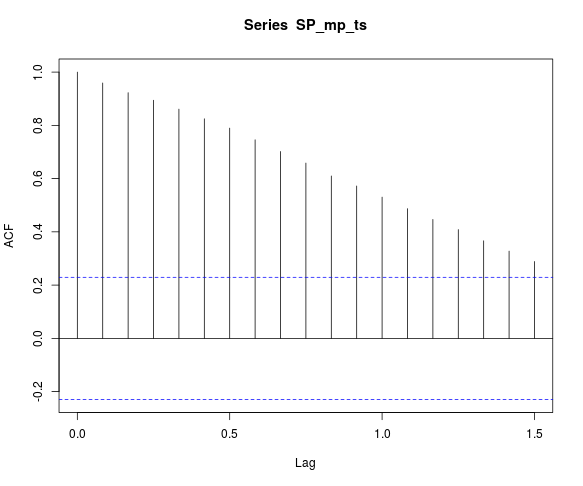
\includegraphics[width=.95\linewidth]{ACF_pr.png}
  	\caption{The ACF of prices.}
    %\label{fig2:sub1}
	\end{subfigure}%
	\hspace{1em}
	\begin{subfigure}{.45\textwidth}
  	\centering
  	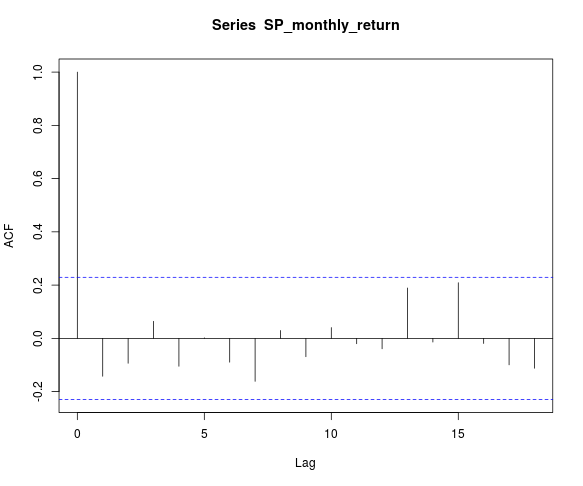
\includegraphics[width=.95\linewidth]{ACF_re.png}
  	\caption{The ACF of Returns.}
 	%\label{fig2:sub2}
	\end{subfigure}
\caption{Autocorrelation Function Plots for the S\&P 500.}
\end{figure}

Given the results of the Box test, returns of the index are stationary while the price is not. Therefore, predictions cannot be made for returns using historical data, but predictive methods can be applied to prices.

\subsection*{ARIMA on Prices}
An Autoregressive Integrated Moving Average (ARIMA) was applied to the prices of the index and the the best model was determined to be ARIMA(1,1,0), see Table 1, Appendix D. The fitted ARIMA model was used for to predict the price of the market over the next two months, see Table 5.

\begin{small}
\vspace{1em}
\begin{minipage}{\linewidth}
\begin{center}
\begin{tabular}{ |P{2.2cm}||P{2.2cm}|P{2.2cm}|  }
 \hline
 \multicolumn{3}{|c|}{\textbf{Prediction Result of ARIMA Mode}} \\
 \hline
  Month &  2015 Dec &  2016 Jan \\
 \hline
Predicted Price&   2087.87 &  2087.98 \\
SE & 55.48 & 74.45  \\
 \hline
\end{tabular}
\bigskip \\
Table 5. ARIMA predictions. Note the market is expected to remain stationary.
\end{center}
\end{minipage}
\end{small}


\subsection*{Decomposition}
The decomposition method is used to extract additional information on the trend and seasonality of the S\&P 500, see Figure 5.

\begin{figure}[H]
\centering
	\begin{subfigure}{.45\textwidth}
  	\centering
  	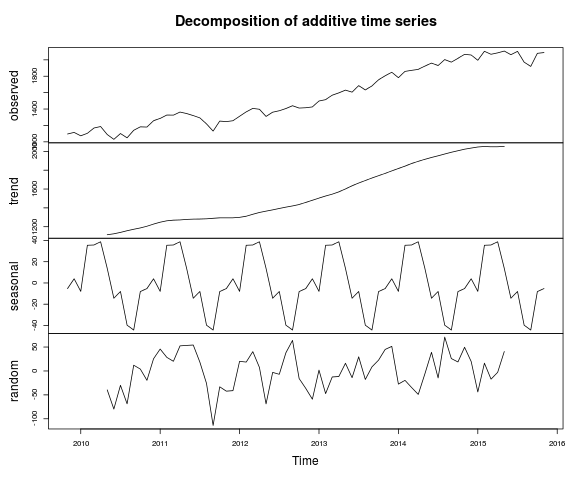
\includegraphics[width=.95\linewidth]{Decompsition_pr.png}
  	\caption{Decomposition of the Price.}
    %\label{fig2:sub1}
	\end{subfigure}%
	\hspace{1em}
	\begin{subfigure}{.45\textwidth}
  	\centering
  	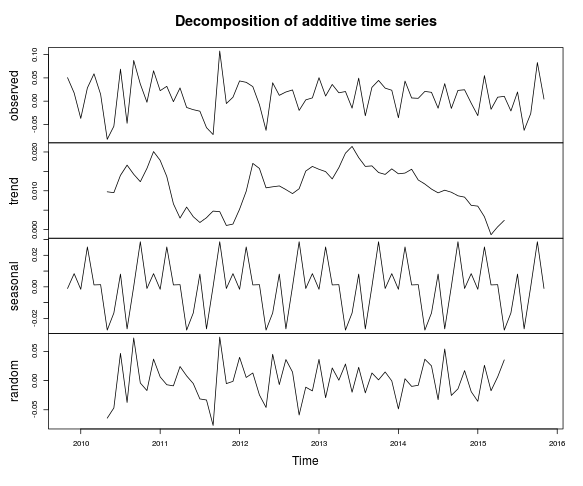
\includegraphics[width=.95\linewidth]{Decompsition_re.png}
  	\caption{Decomposition of the Return.}
 	%\label{fig2:sub2}
	\end{subfigure}
	\caption{Decomposition Plots for the S\&P 500.}
\end{figure}

The price of the S\&P 500 is increasing, however the rate of increase is slowing. In addition, January and September appear to be favorable times to increase holdings while holdings should be reduced in February or March. Given this information, investors stand to gain in the short term. However, given historically poor market performance in February or March and the slowing rate of gains, caution should be used in the long term.

\newpage

\section*{Appendix}

\subsection*{A. Assets}
\begin{figure}[H]
	\centering
  	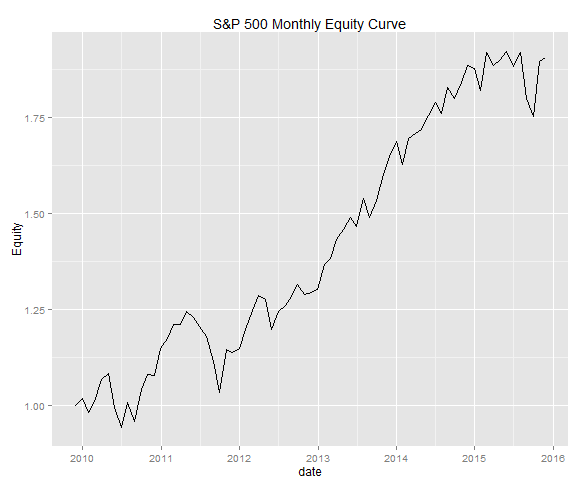
\includegraphics[width=.85\linewidth]{SP500_Equity_Curve}
  	\centering
  	\caption{Equity Curve for the S\&P 500.}
\end{figure}

\begin{figure}[H]
	\centering
  	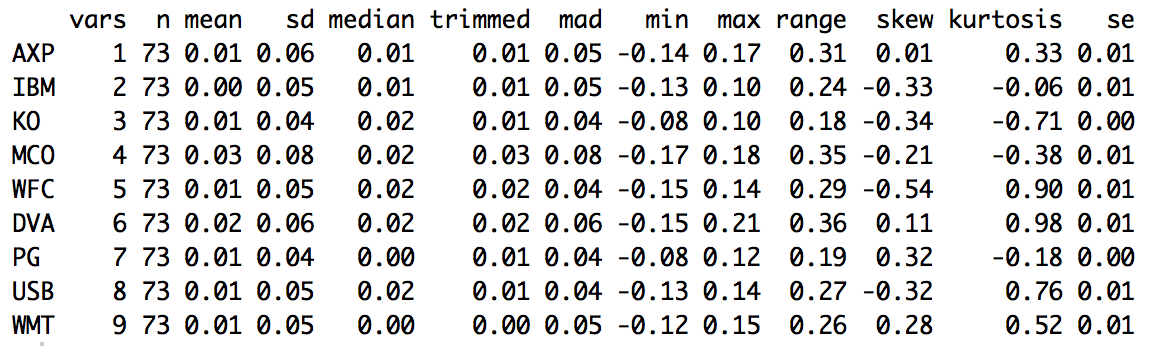
\includegraphics[width=.85\linewidth]{means_sd_skewness_kurtosis}
  	\centering
  	\caption{Summary of sample statistics of nine large capitalization assets}
\end{figure}

We can see that six of the assets have mean return of 0.01. IBM has the lowest mean return of
0.00 with standard deviations of 0.05. Even though MCO has the highest mean return of 0.03, it
also has the highest standard deviation of 0.08. AXO has the least skewed because it has the
lowest absolute value of skewness coefficient. WFC has both a high skewness coefficient and a
high kurtosis coefficient.

\begin{figure}[H]
	\centering
  	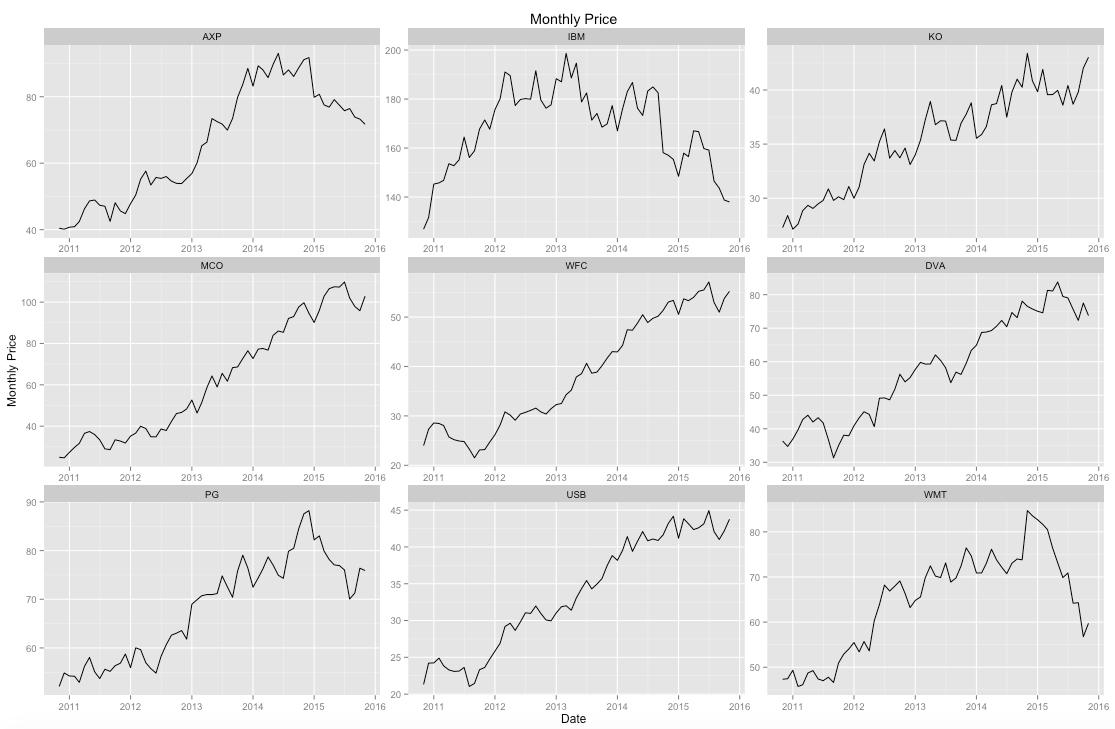
\includegraphics[width=.85\linewidth]{monthly_price_adjusted}
  	\centering
  	\caption{Adjusted monthly prices of each of the nine large capitalization assets.}
\end{figure}

\begin{figure}[H]
	\centering
  	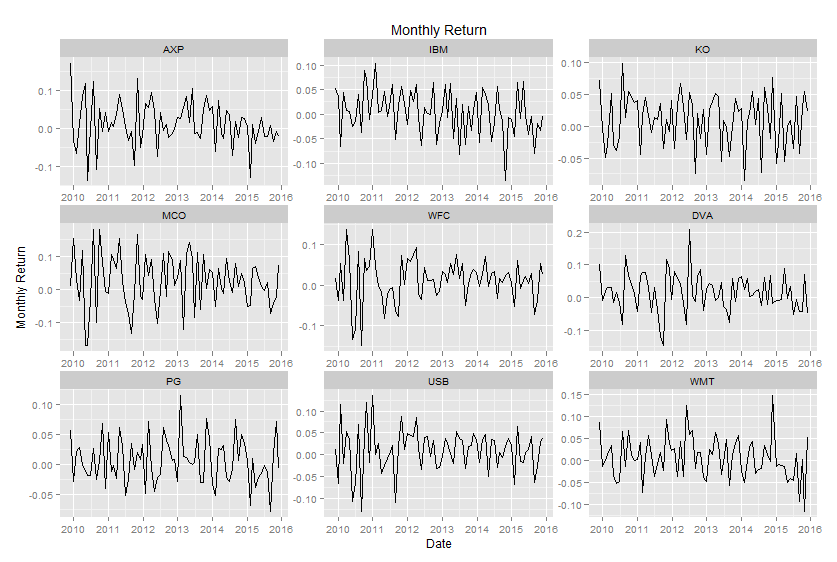
\includegraphics[width=.85\linewidth]{monthly_returns}
  	\centering
  	\caption{Monthly returns of each of the nine large capitalization assets.}
\end{figure}

\begin{figure}[H]
	\centering
  	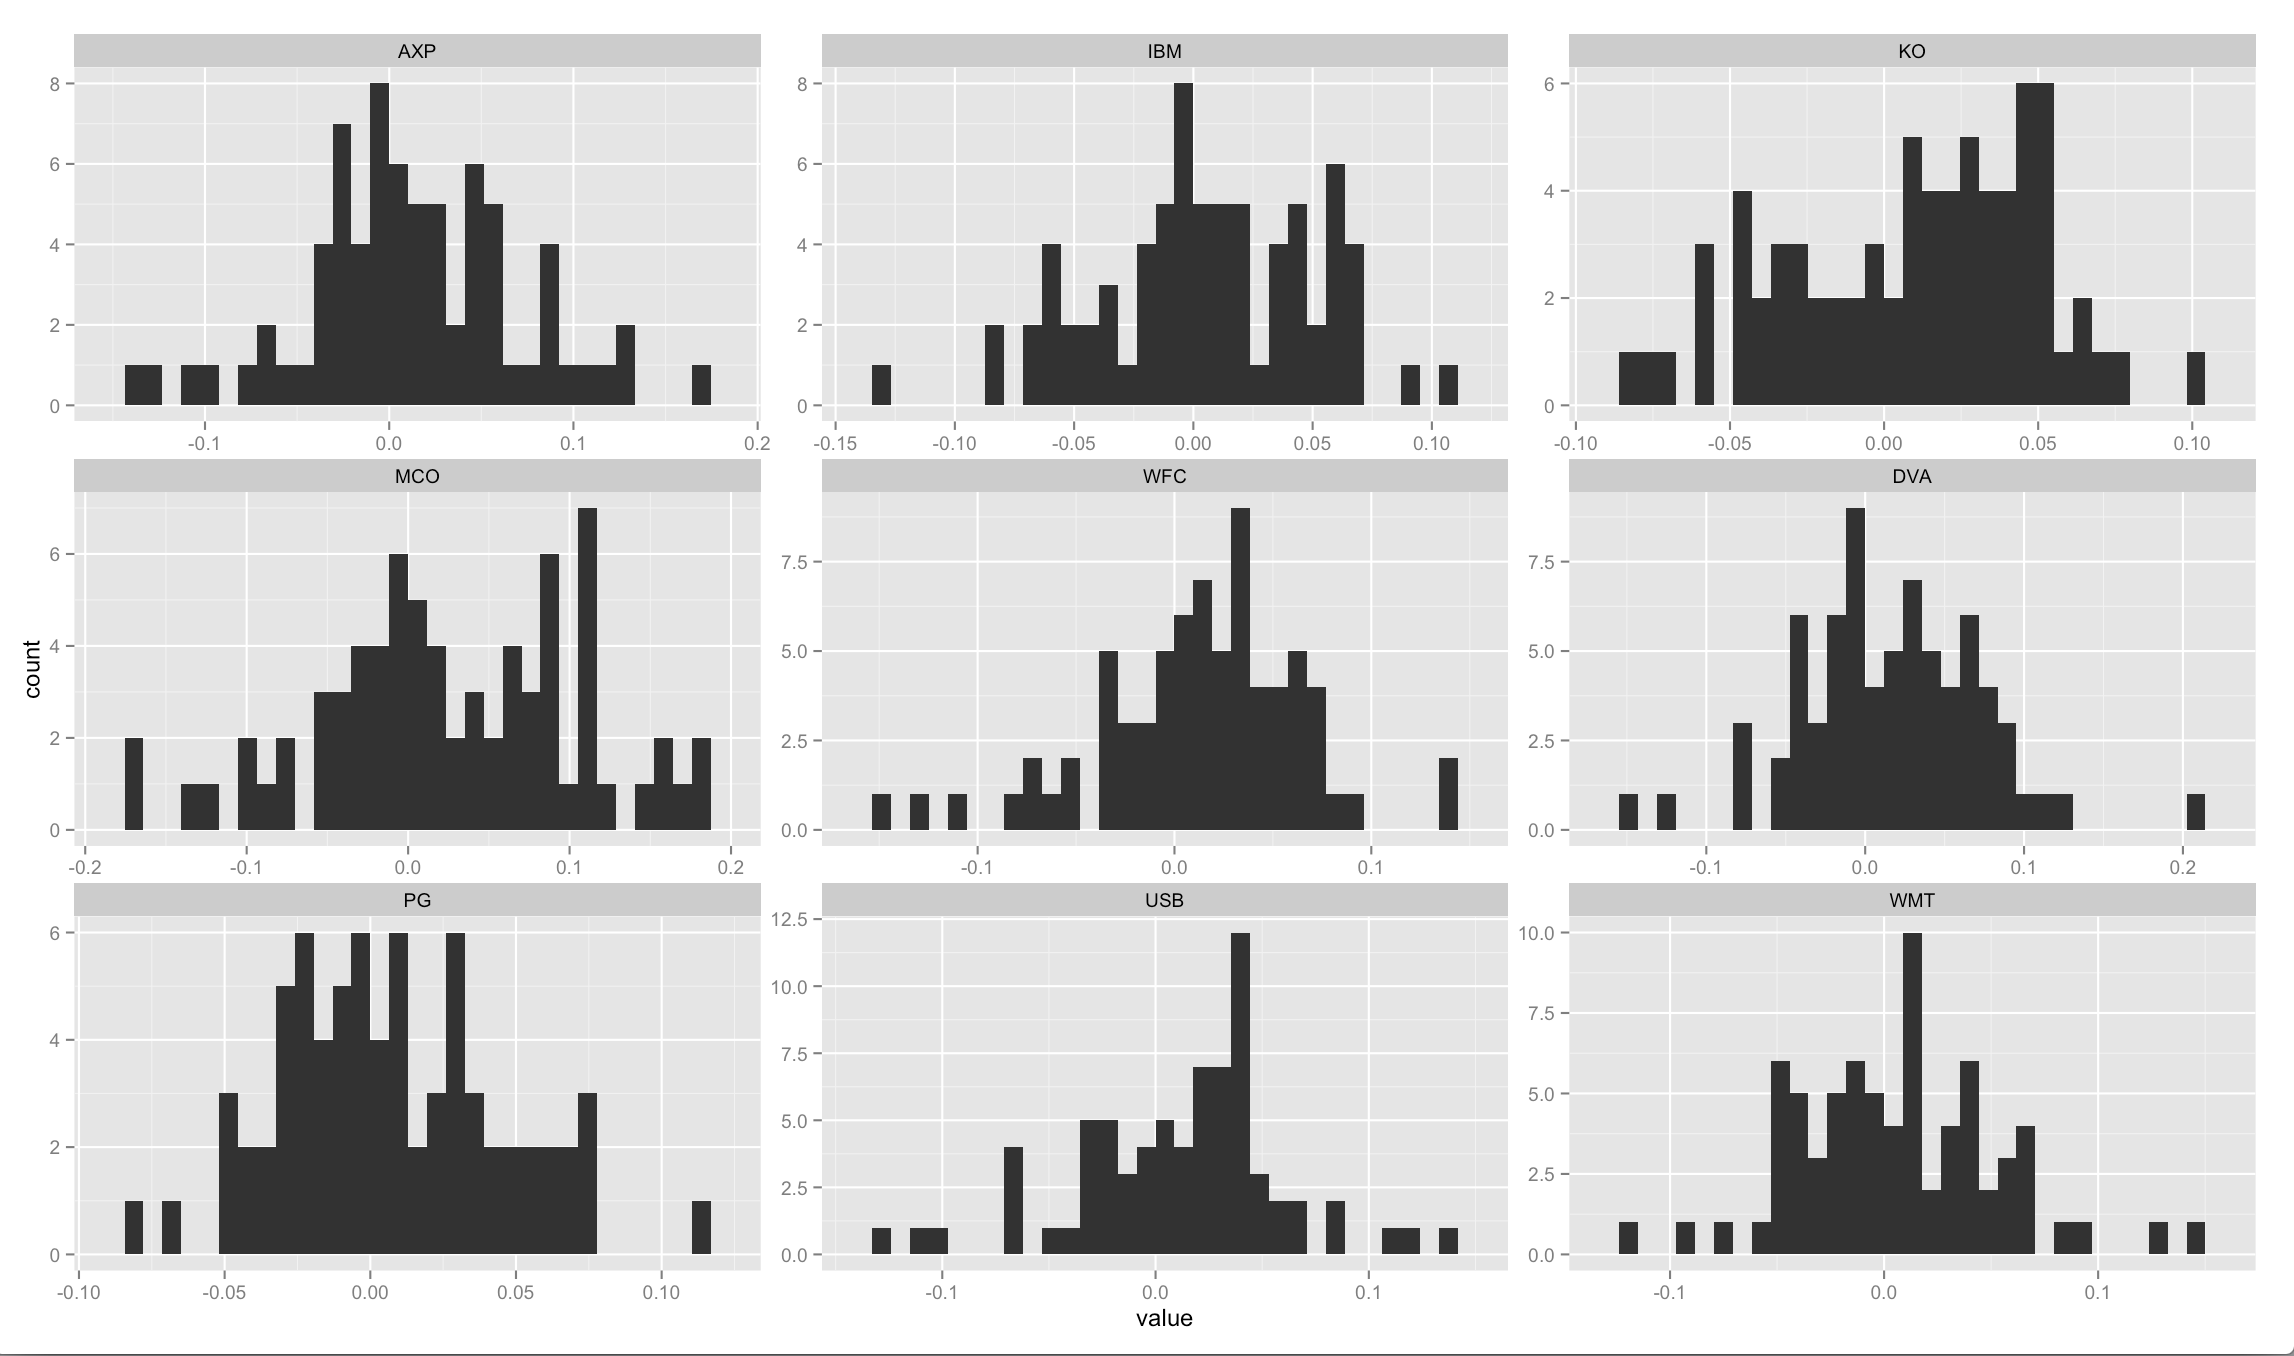
\includegraphics[width=.85\linewidth]{histograms}
  	\centering
  	\caption{Histograms of assets returns.}
\end{figure}

\begin{figure}[H]
	\centering
  	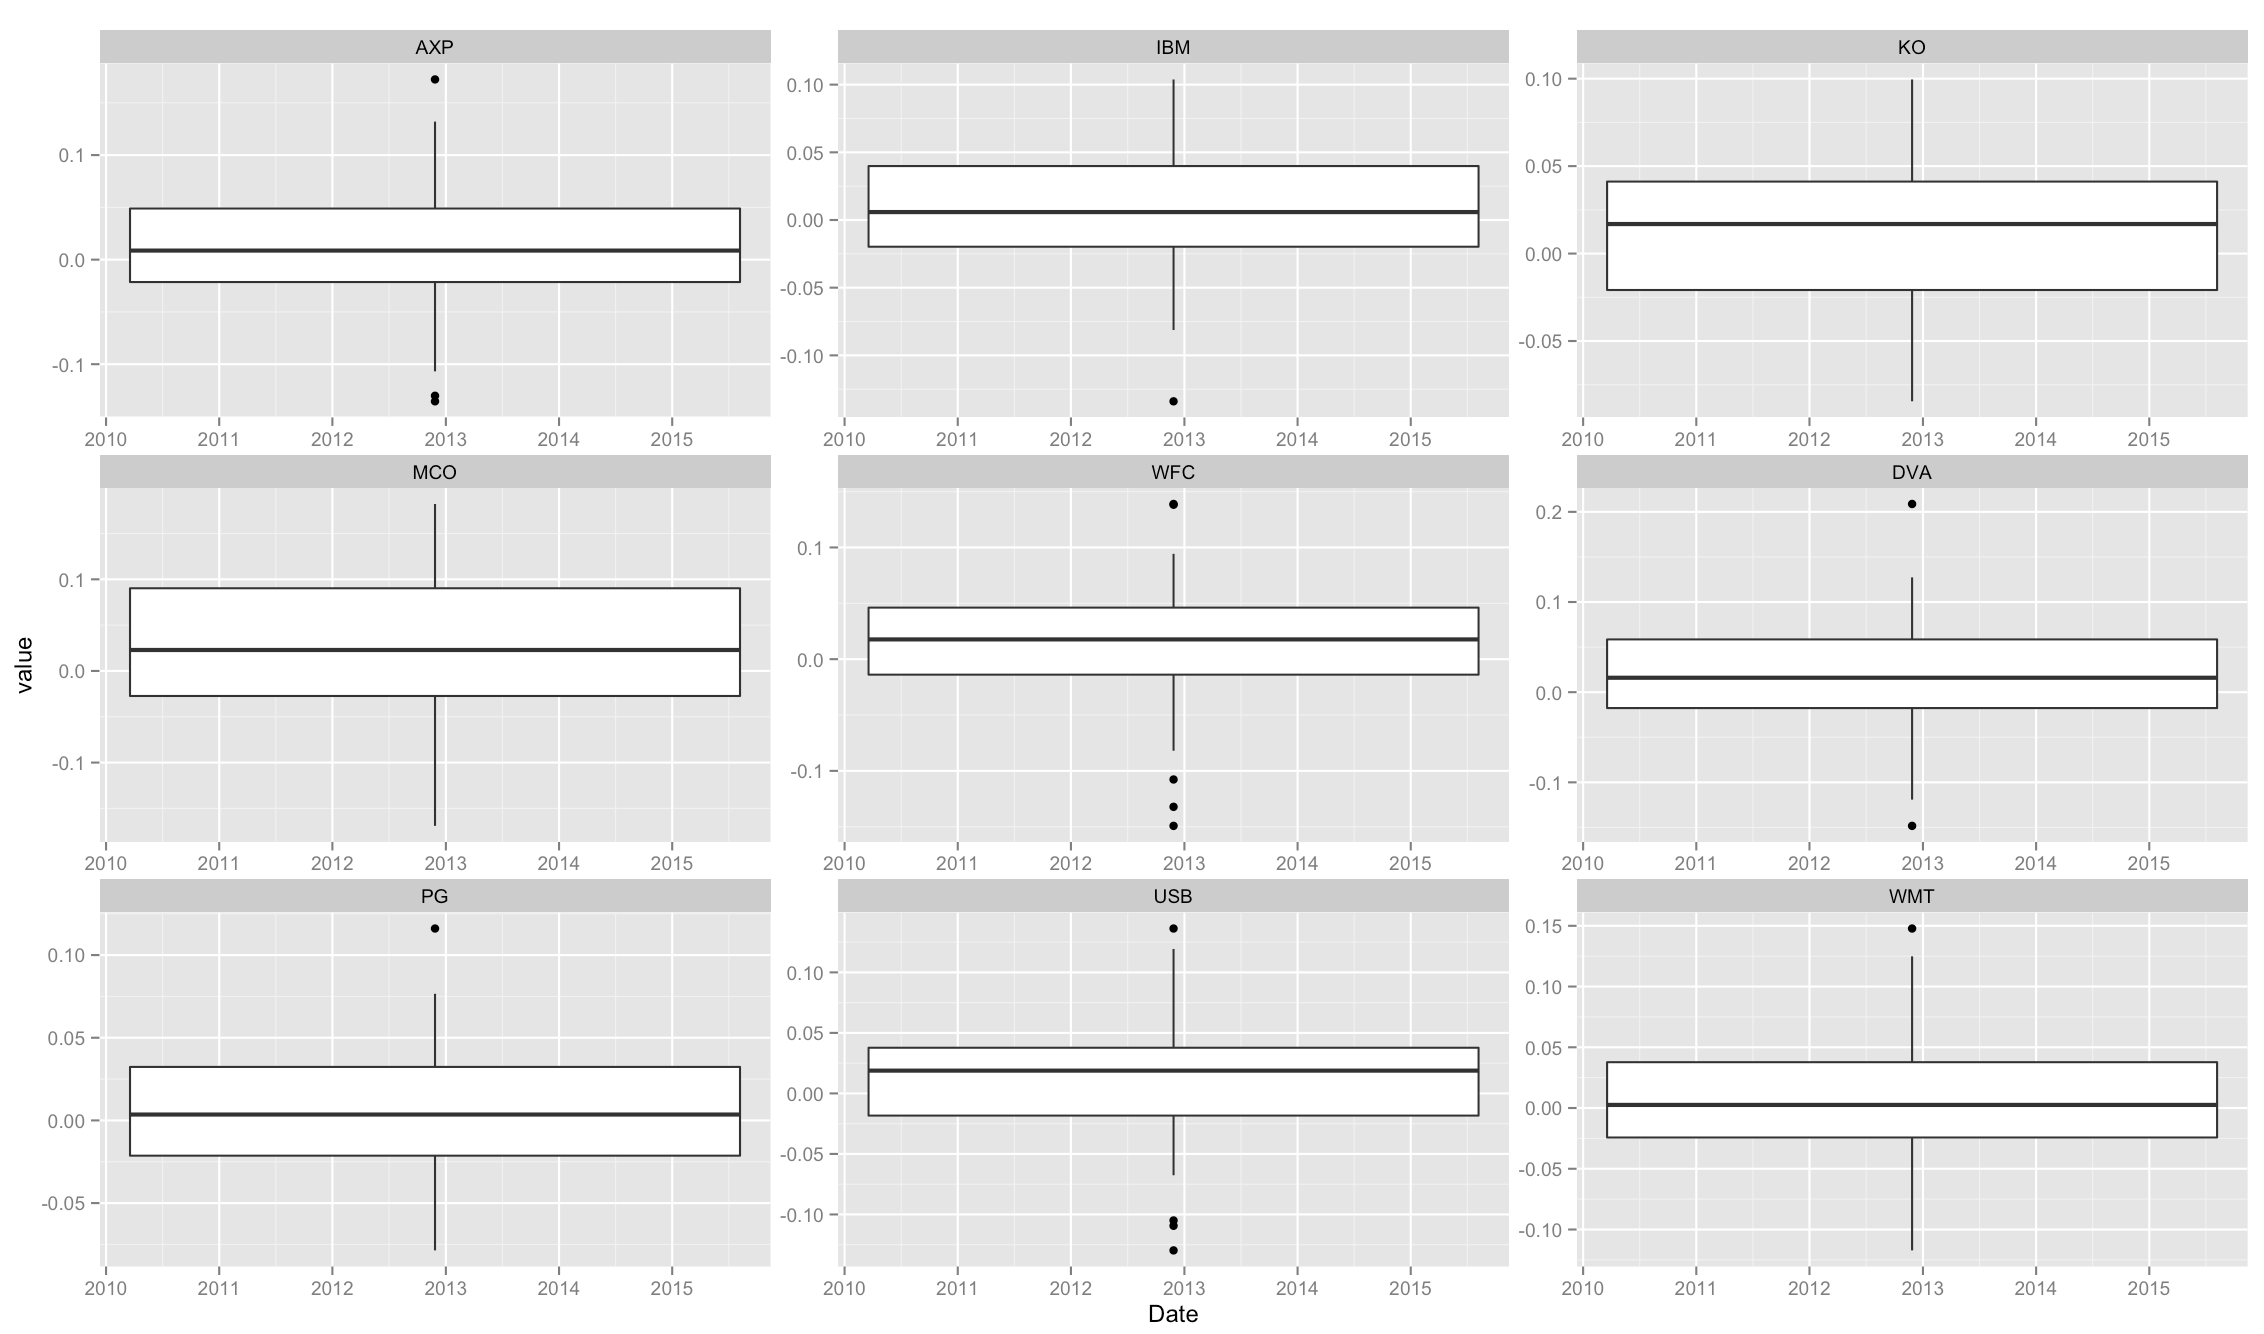
\includegraphics[width=.85\linewidth]{boxplots}
  	\centering
  	\caption{Boxplots of assets returns.}
\end{figure}

\begin{figure}[H]
	\centering
  	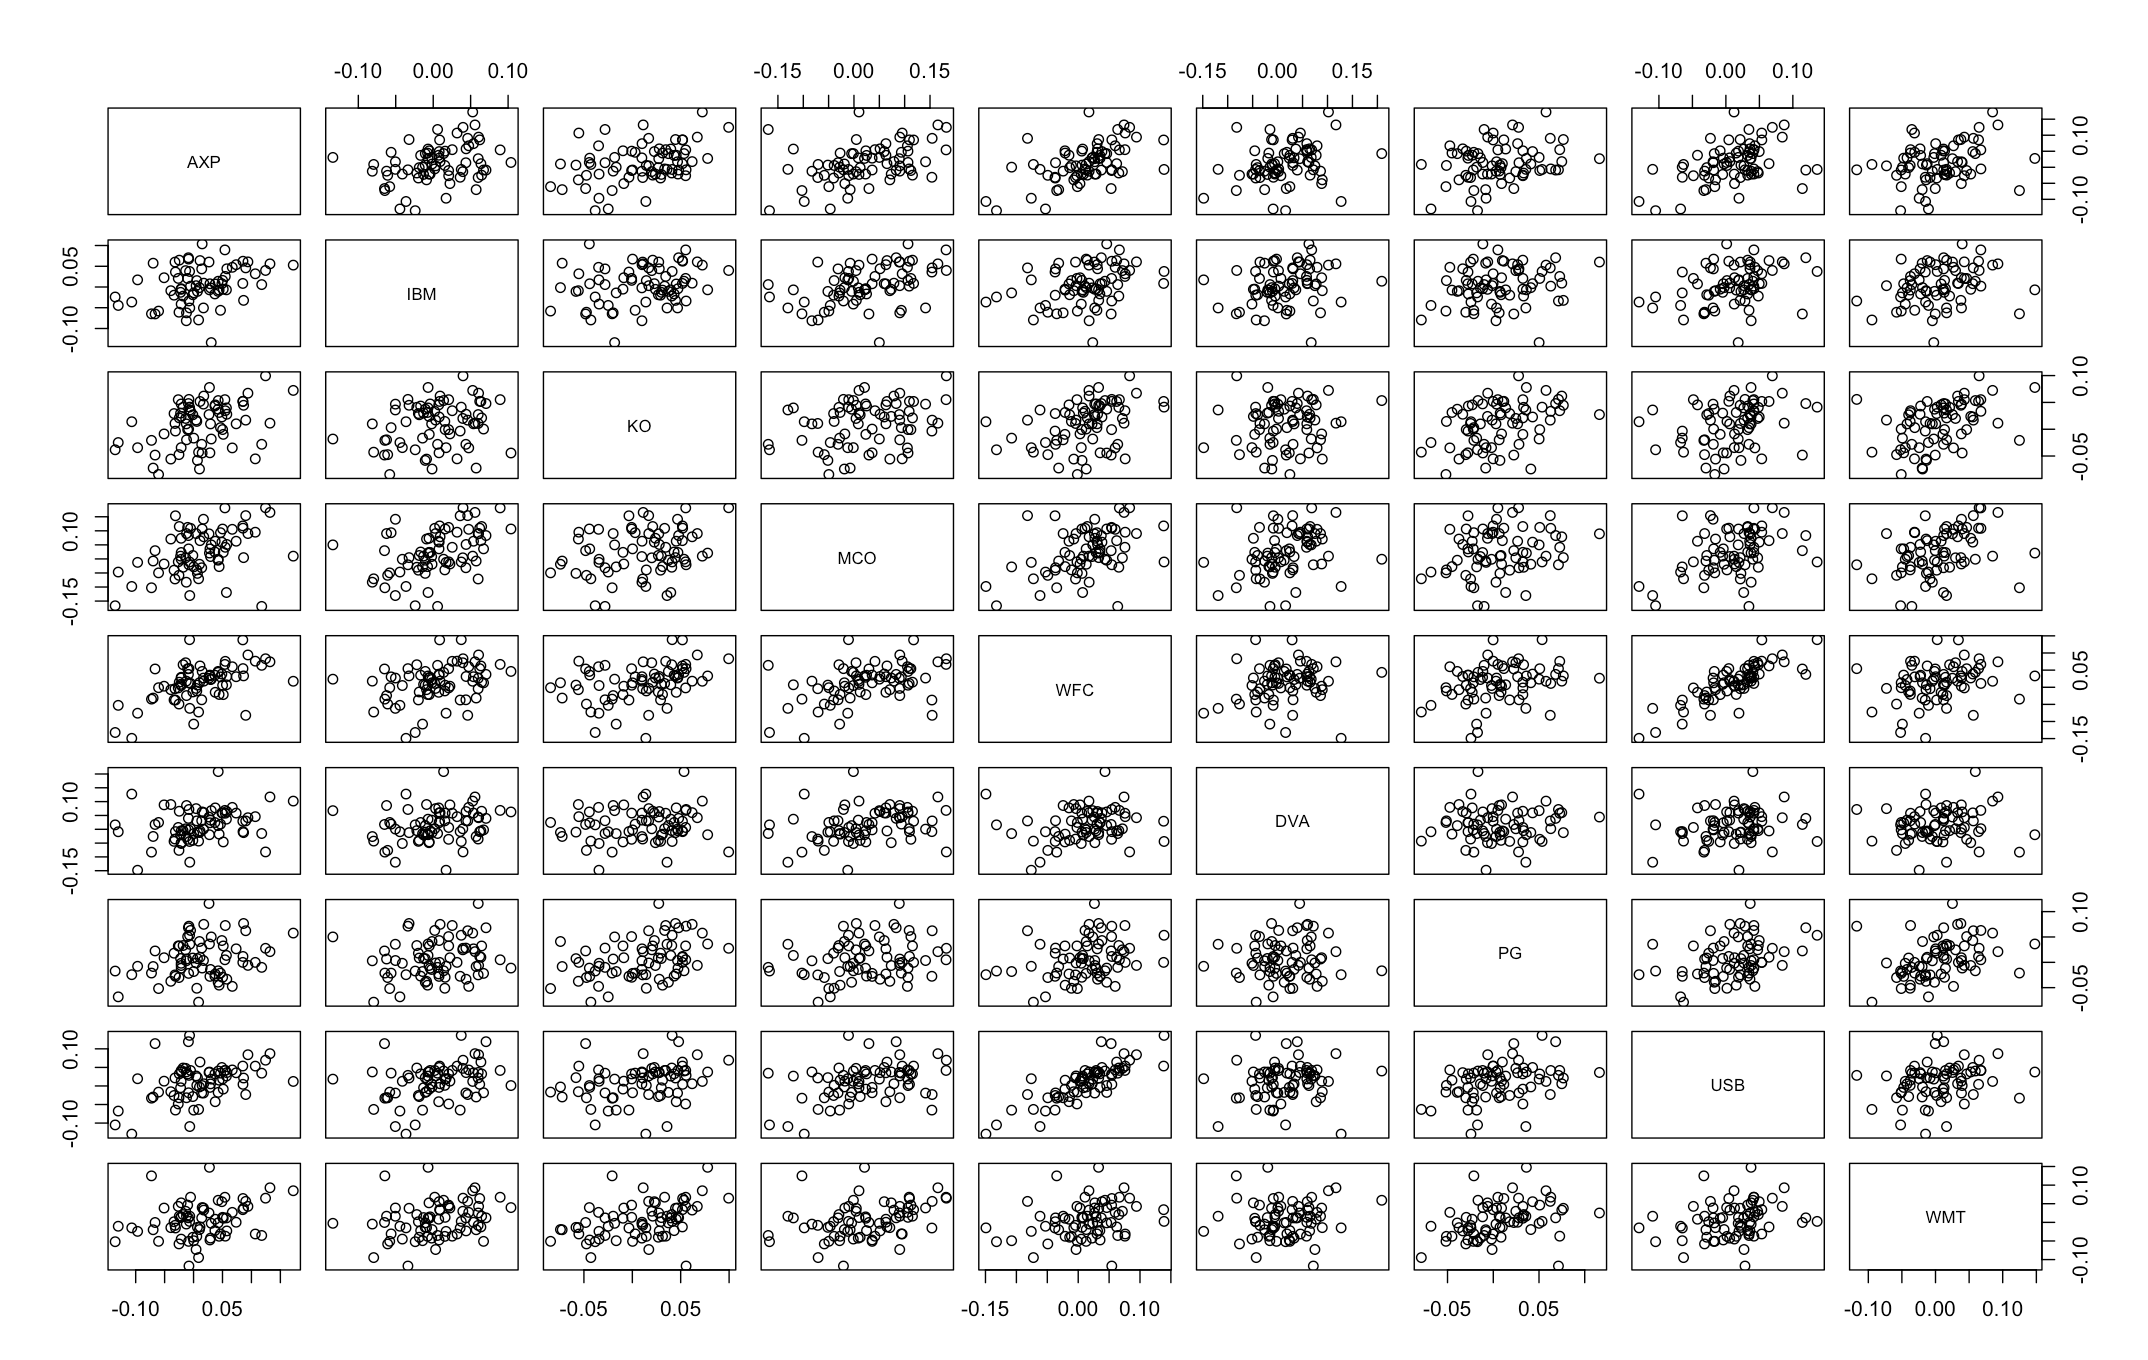
\includegraphics[width=.85\linewidth]{pairwise_scatter_plots}
  	\centering
  	\caption{Pairwise scatter plots between assets returns.}
\end{figure}

Note that no outliers are seen in the scatterplots. Changes in return in WFC show a positive
relationship with changes in return in USB. So they are useful for predicting changes in the
return of each other. The correlations between changes in return in other variables are not as
strong. Next, we look at the sample covariance matrix, see Figure 13.

\begin{figure}[H]
	\centering
  	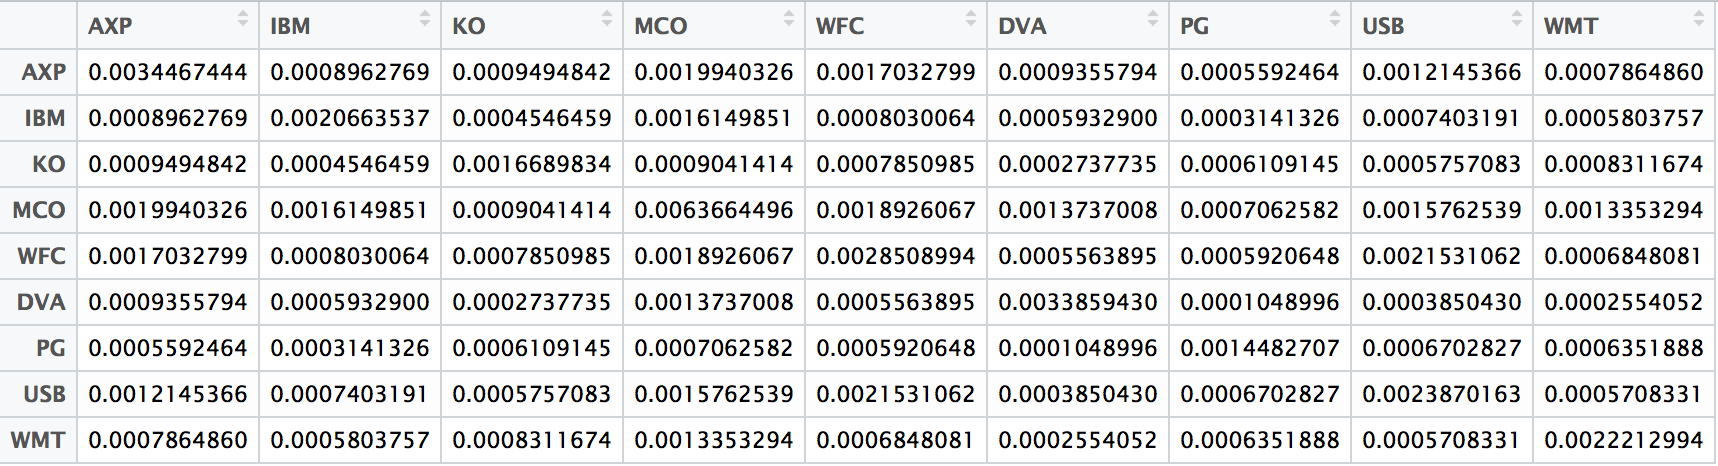
\includegraphics[width=.85\linewidth]{covariance_matrix}
  	\centering
  	\caption{Sample covariance matrix of the returns on the nine assets.}
\end{figure}

Notice that WFC and USB have the strongest correlation. It makes sense because WFC (Wells
Fargo \& Co) and USB (U.S. Bancorp) are both financial services company, so their returns tend
to move together.

\begin{figure}[H]
	\centering
  	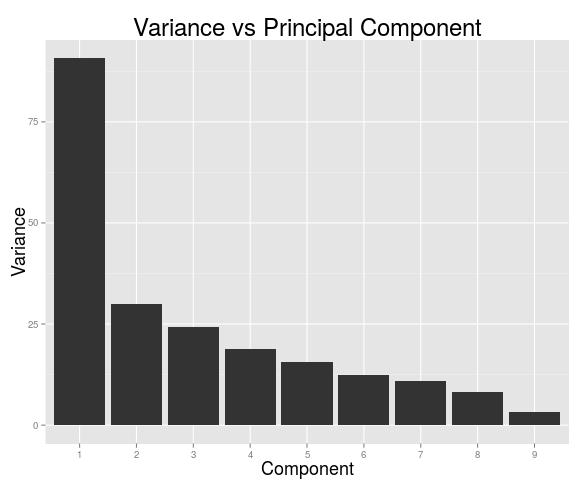
\includegraphics[width=.55\linewidth]{PCA}
  	\centering
  	\caption{Scree Plot of the Variance of the Principle Components. The first component accounts for 42\% of the variance whereas 8 components are required to account for $>95\%$ of the total variance.}
\end{figure}


\begin{figure}[H]
	\centering
  	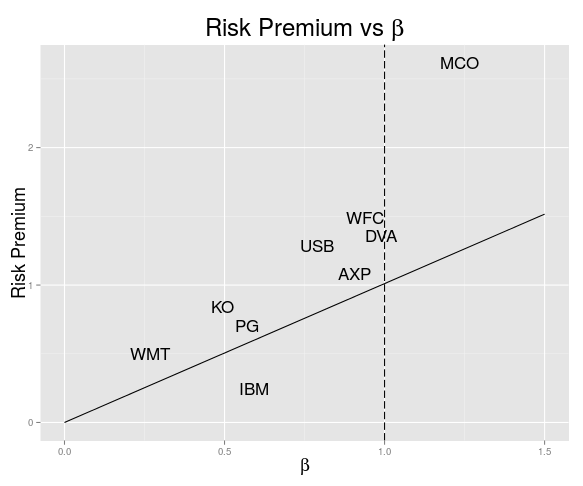
\includegraphics[width=.55\linewidth]{Risk_Premium_vs_Beta}
  	\centering
  	\caption{Asset Risk Premiums Plotted with the security Market Line (SML) and dashed line indicating the market. All assets were found to obey the Capital Asset Pricing Model.}
\end{figure}


\begin{small}
\begin{minipage}{\linewidth}
\begin{center}
\begin{tabular}{ |P{0.8cm}|P{0.8cm}|P{0.8cm}|P{0.8cm}|P{0.8cm}|P{0.8cm}|P{0.8cm}|P{0.8cm}|P{0.8cm}|  }
 \hline
 \multicolumn{9}{|c|}{\textbf{Annualized Asset Sharpe Ratio}} \\
 \hline
  AXP &  IBM &   KO &  MCO &  WFC &  DVA &   PG &  USB &  WMT \\
 \hline
0.75 & 0.18 & 0.73 & 1.31 & 1.20 & 0.79 & 0.62 & 1.10& 0.36 \\
 \hline
\end{tabular}
\bigskip \\
Table 6. Asset Sharpe Ratios, note financial and financial services companies tend to have higher values.
\end{center}
\end{minipage}
\end{small}

\subsection*{B. Asset Allocations}

\begin{small}
\begin{minipage}{\linewidth}
\begin{center}
\begin{tabular}{ |P{2.2cm}||P{2.2cm}|P{2.2cm}|P{2.2cm}|P{2.2cm}|  }
 \hline
 \multicolumn{5}{|c|}{\textbf{\% Asset Weight by Portfolio Type}} \\
 \hline
 Ticker Symbol  &  Min Variance  (No Shorts) &  Min Variance &   Tangency (No Shorts)  &    Tangency  \\
 \hline
AXP&  2.8&  6.3&  0.0&  -9.8\\
IBM&  16.6& 19.4&  0.0& -10.0\\
KO&  19.5& 17.2&  21.0&  28.1\\
MCO&  0.0& -8.7&  33.4&  32.4\\
WFC& 0.0& -5.2&  30.3&  26.7\\
DVA&  9.7& 12.9&  0.7&   5.8\\
PG&  24.5& 25.8&  2.0&  10.3\\
USB&  15.3& 19.4&  12.6&  20.6\\
WMT&  11.5& 13.0& 0.00&  -4.2\\
 \hline
\end{tabular}
\bigskip \\
Table 7. Asset allocation, note both tangency portfolios depend heavily on companies in the finance/financial services sectors (MCO, WFC, and UBS).
\end{center}
\end{minipage}
\end{small}


\begin{small}
\begin{minipage}{\linewidth}
\begin{center}
\begin{tabular}{ |P{2.5cm}||P{2.5cm}|P{2.5cm}|  }
 \hline
 \multicolumn{3}{|c|}{\textbf{\% Asset Weights for 12\%/year Return Portfolios}} \\
 \hline
  Ticker Symbol &  Efficient Portfolio &  Tangency w/ Risk Free \\
 \hline
Risk Free & 0.0 &  40.9 \\
AXP  &      1.8 & 0.0\\
IBM  &      6.5 &  0.0 \\
KO   &     20.8 &  12.4 \\
MCO  &      3.9 &  19.7 \\
WFC  &      4.3 &  17.9 \\
DVA  &     11.1 &  0.4 \\
PG   &     21.6 &  1.17 \\
USB  &     21.2 &  7.42 \\
WMT  &      8.7 &  0.0 \\
 \hline
\end{tabular}
\bigskip \\
Table 8. Asset allocation for portfolios targeting 12\% annualized returns. Note the portfolio that combines the tangency portfolio and T-Bills was constructed from a previously derived tangency portfolio but does not suffer as much from the same potential lack of asset diversity due to the large allocation of funds to the risk free asset.
\end{center}
\end{minipage}
\end{small}

\newpage


\begin{framed}
\center
\textbf{Bootstrap Estimates of ES and VaR}

\begin{small}
\begin{minipage}{\linewidth}
\begin{center}
\begin{tabular}{ |P{2.2cm}||P{2.2cm}|P{2.2cm}|P{2.2cm}|P{2.2cm}|  }
 \hline
 \multicolumn{5}{|c|}{\textbf{Parametric VaR Estimates}} \\
 \hline
 Ticker Symbol  &  $\widehat{VaR}^{par}(0.05) (\$)$ &  95\% CI $(\$)$  &   BIAS$_{boot}$  &    SE$_{boot}$ \\
 \hline
AXP  & 7101&         (5401,        9784)& 1.24e-3 & 1.08e-2 \\
IBM  & 7265&         (5610,         9972)& 1.01e-3& 1.03e-2 \\
KO  &    5675&        (4082,         7371)& 7.71e-4& 8.55e-3 \\
MCO  &   8787 &        (6460,       11910)& 1.64e-3& 1.34e-2\\
WFC  &   5569  &       (4003,        7590)& 7.85e-4& 9.13e-3\\
DVA  &   8405   &      (6257,       11722)& 1.35e-3& 1.32e-2\\
PG  &    5754    &     (4610,        7300)& 8.71e-4& 6.68e-3\\
USB  &   5350     &    (3767,        7771)& 9.64e-3& 9.57e-3\\
WMT  &   7410      &   (5773,        9631)& 8.00e-4& 9.63e-3\\
 \hline
\end{tabular}
\bigskip \\

\end{center}
\end{minipage}
\end{small}

\begin{small}
\begin{minipage}{\linewidth}
\begin{center}
\begin{tabular}{ |P{2.2cm}||P{2.2cm}|P{2.2cm}|P{2.2cm}|P{2.2cm}|  }
 \hline
 \multicolumn{5}{|c|}{\textbf{Parametric Expected Shortfall Estimates}} \\
 \hline
 Ticker Symbol  &  $\widehat{ES}^{par}(0.05) (\$)$ &  95\% CI $(\$)$  &   BIAS$_{boot}$  &    SE$_{boot}$ \\
 \hline
AXP & 9180 &         (7202,      12318)& -1.13e-3& 1.22e-2 \\
IBM & 9173  &       (7300,       11957)& -7.87e-4& 1.16e-2 \\
KO  & 7331   &      (5571,         9492)& -1.36e-3& 9.97e-3 \\
MCO & 11685   &      (9299,        15126)& -2.17e-3& 1.46e-2 \\
WFC & 7362     &    (5678,         9709)& -1.01e-3& 1.02e-2\\
DVA & 10884     &   (8364,        14643)& -1.50e-3& 1.54e-2\\
PG &  7395       &  (6063,         9210)& -9.08e-4& 7.89e-3\\
USB & 7036        & (5148,         9760)& -1.18e-3& 1.12e-2\\
WMT & 9419        & (7544,        12148)& -1.82e-3& 1.15e-2\\
 \hline
\end{tabular}
\bigskip \\

\end{center}
\end{minipage}
\end{small}

\begin{small}
\begin{minipage}{\linewidth}
\begin{center}
\begin{tabular}{ |P{2.2cm}||P{2.2cm}|P{2.2cm}|P{2.2cm}|P{2.2cm}|  }
 \hline
 \multicolumn{5}{|c|}{\textbf{Nonparametric VaR Estimates}} \\
 \hline
 Ticker Symbol  &  $\widehat{VaR}^{np}(0.05) (\$)$ & 95\% CI $(\$)$  &   BIAS$_{boot}$  &    SE$_{boot}$ \\
 \hline
AXP&   7000  &       (4086,        13019)&  3.18e-3& 1.85e-2\\
IBM&   6532   &      (5913,        13396)& -3.82e-3& 1.30e-2\\
KO &   5893    &     (4780,         8448)& -2.48e-3& 1.03e-2\\
MCO &  8392     &    (7069,        13034)& -1.32e-3& 2.04e-2\\
WFC &  6225      &   (3792,         8199)&  3.04e-3& 1.36e-2\\
DVA &  7677       &  (4614,        14827)&  3.59e-3& 2.54e-2\\
PG  &  5122        & (3785,         7862)&  7.10e-4& 9.62e-3\\
USB &  4927      &   (3241,        10936)& -5.47e-4& 1.54e-2\\
WMT &  5870       &  (4755,        11721)& -4.23e-3& 1.67e-2\\
 \hline
\end{tabular}
\bigskip \\

\end{center}
\end{minipage}
\end{small}

\begin{small}
\begin{minipage}{\linewidth}
\begin{center}
\begin{tabular}{ |P{2.2cm}||P{2.2cm}|P{2.2cm}|P{2.2cm}|P{2.2cm}|  }
 \hline
 \multicolumn{5}{|c|}{\textbf{Nonparametric Expected Shortfall Estimates}} \\
 \hline
 Ticker Symbol  &  $\widehat{ES}^{np}(0.05) (\$)$ &  95\% CI $(\$)$  &   BIAS$_{boot}$  &    SE$_{boot}$ \\
 \hline
AXP&  9990&         (5674,        13019)& 2.54e-2& 3.39e-2\\
IBM&  9824 &        (6698,       13396)& 2.46e-2& 3.26e-2\\
KO &  7707  &       (4224,         8448)& 2.01e-2& 2.36e-2\\
MCO& 11750   &      (6247,       13034)& 3.15e-2& 3.66e-2\\
WFC & 7676    &     (4100,       8199)& 2.02e-2& 2.31e-2\\
DVA& 11675     &    (6300,       14827)& 2.97e-2& 3.89e-2\\
PG  & 6614      &   (3667,         7862)& 1.64e-2& 2.10e-2\\
USB & 8008       &  (5286,        10936)& 2.09e-2& 2.66e-2\\
WMT & 9491        & (5861,        11721)& 2.48e-2& 3.06e-2\\
 \hline
\end{tabular}
\bigskip \\

\end{center}
\end{minipage}
\end{small}
\end{framed}

\begin{small}
\center
Table 9. Nonparametric and Parametric monthly ES and VaR estimates assuming \$100,000.00 invested in each asset. Confidence intervals, bias and standard error estimated by bootstrap with B = 2000 resamplings.
\end{small}

\subsection*{C. Copulas}
Five parametric copulas were fit to the returns: Gaussian, t, Gumbel, Frank, and Clayton.

Since the marginal distributions of the nine assets are unknown, to minimize biases in the estimated parameters of the copula, we applied pseudo-maximum likelihood estimation, where the marginal distributions are estimated nonparametrically. The results are in Table 10.

By comparing the five copula’s AIC, we see that t-copula fits best since it minimizes AIC. It’s also noted that Gaussian Copula’s AIC is only slightly larger than t-copula’s, which means the joint distribution of the returns is approximately normally distributed. This conclusion can be verified by Figure 16. The Q-Q plots of the nine assets are all approximately linear. More
precisely, from the S shape of the Q-Q plots, we can conclude that the marginal distribution of the nine assets have lighter tail than normal distribution.

\begin{small}
\vspace{1em}
\begin{minipage}{\linewidth}
\begin{center}
\begin{tabular}{ |P{3.5cm}||P{3.5cm}|P{3.5cm}|P{3.5cm}|  }
 \hline
 \multicolumn{4}{|c|}{\textbf{Copula Fit}} \\
 \hline
Copula Family &  Estimates& Maximized log-likelihood&  AIC  \\
 \hline
Gaussian & $\hat{\rho} $: between each pair of assets, values omitted & 119.325 & -220.650\\
 \hline
t & $\hat{\rho} $: between each pair of assets, values omitted $\hat{\nu} = 21.613$  & 120.477 & -222.955\\
 \hline
Gumbel & $\hat{\theta} = 1.239$ & 48.452 & -78.904 \\
 \hline
Frank & $\hat{\theta} = 1.707$ & 49.355 & -80.709 \\
 \hline
Clayton & $\hat{\theta} = 0.377$ & 54.982 & -91.964 \\
 \hline
\end{tabular}
\bigskip \\
Table 10. Summary of estimates of copula parameters, nine assets.
\end{center}
\end{minipage}
\end{small}

\begin{figure}[H]
	\centering
  	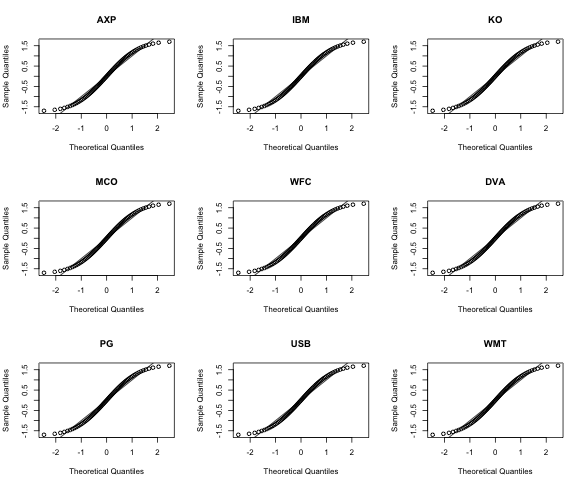
\includegraphics[width=.85\linewidth]{QQ-plot}
  	\centering
  	\caption{Q-Q plots of the nine large market capitalization assets.}
\end{figure}
Although t-Copula fits best the joint distribution of the nine assets, it may not fit best the joint
distribution of subsets of the nine assets. Take PG and WMT as an example. Table 2 shows the
summary of estimates of their copula parameters.


\begin{small}
\vspace{1em}
\begin{minipage}{\linewidth}
\begin{center}
\begin{tabular}{ |P{3.5cm}||P{3.5cm}|P{3.5cm}|P{3.5cm}|  }
 \hline
 \multicolumn{4}{|c|}{\textbf{PG and WMT Copula Fit}} \\
 \hline
Copula Family &  Estimates& Maximized log-likelihood&  AIC  \\
 \hline
Gaussian & $\hat{\rho} = 0.442$ & 6.778 & -9.556 \\
 \hline
t & $\hat{\rho} = 0.468$ $\hat{\nu}= 7.375$ & 7.635 & -11.269 \\
 \hline
Gumbel & $\hat{\theta} = 1.366$ & 5.316 & -6.633 \\
 \hline
Frank & $\hat{\theta} = 3.137$ & 8.366 & -12.731 \\
 \hline
Clayton & $\hat{\theta} = 0.782$ & 7.802 & -11.605 \\
 \hline
\end{tabular}
\bigskip \\
Table 11. Summary of estimates of copula parameters, PG and WMT.
\end{center}
\end{minipage}
\end{small}

We can see that instead of t-copula, Frank Copula minimizes AIC of PG and WMT. Figure 17
plots contours of the distribution functions of six copulas: the empirical copula and five
estimated parametric copulas. Since the five estimated parametric copulas’ AIC are quite similar,
their contours of the distribution functions are also similar to each other.

\begin{figure}[H]
	\centering
  	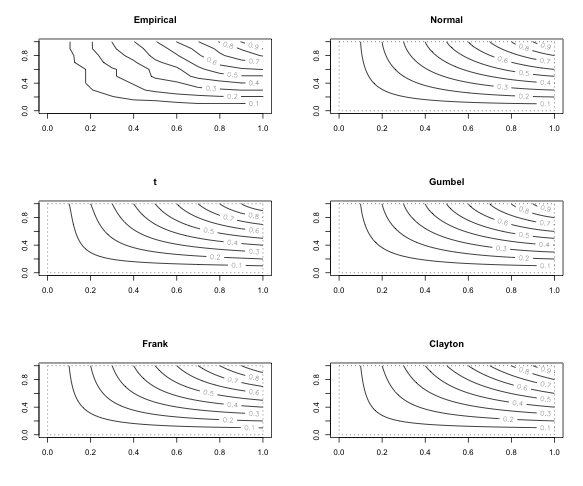
\includegraphics[width=.95\linewidth]{Copula}
  	\centering
  	\caption{Empirical copula, and fitted copulas using five parametric models.}
\end{figure}


\subsection*{D. Time Series}

\begin{figure}[H]
\centering
	\begin{subfigure}{.45\textwidth}
  	\centering
  	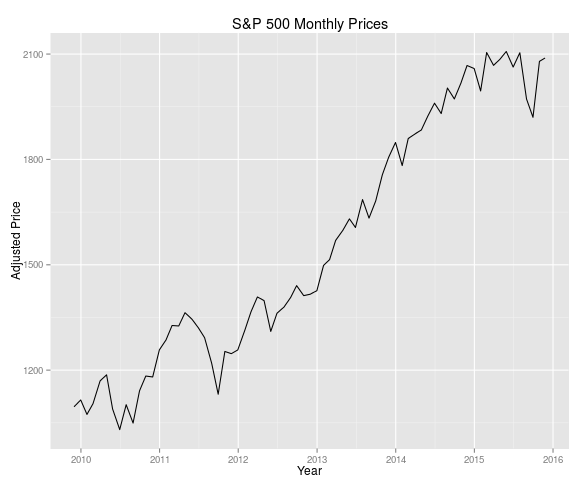
\includegraphics[width=.95\linewidth]{SP500_Price}
  	\caption{The Price of S\&P500 Index}
    %\label{fig2:sub1}
	\end{subfigure}%
	\hspace{1em}
	\begin{subfigure}{.45\textwidth}
  	\centering
  	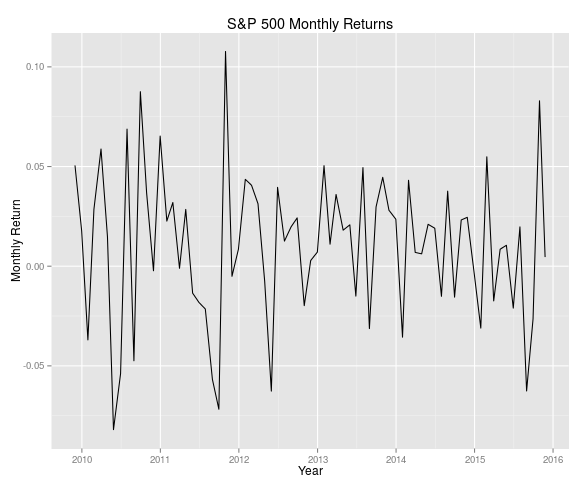
\includegraphics[width=.95\linewidth]{SP500_Return}
  	\caption{The Return of S\&P500 Index.}
 	%\label{fig2:sub2}
	\end{subfigure}
	\caption{S\&P Price and Returns.}
\end{figure}

% Table generated by Excel2LaTeX from sheet 'Sheet1'
\setcounter{table}{11}
\makeatletter
\renewcommand{\thetable}{S\arabic{table}}


\begin{table}[htbp]
  \centering
  \caption{ARIMA Model}
    \begin{tabular}{r}
    \multicolumn{1}{l}{Call:} \\
    \multicolumn{1}{c}{arima(x = SP\_mp\_ts, order = c(1, 1, 0))} \\
    \multicolumn{1}{c}{} \\
    \multicolumn{1}{l}{Coefficients:} \\
    \multicolumn{1}{c}{ar1} \\
    \multicolumn{1}{c}{-0.105} \\
    \multicolumn{1}{c}{s.e.   0.1165} \\
    \multicolumn{1}{c}{} \\
    \multicolumn{1}{c}{sigma$^2$ estimated as 3078:  log likelihood = -391.32,  aic = 786.64 } \\
    \end{tabular}%
%  \label{tab:addlabel}%
\end{table}%

\subsection*{E. Univariate Fitting of Individual Assets}

\begin{figure}[H]
	\centering
  	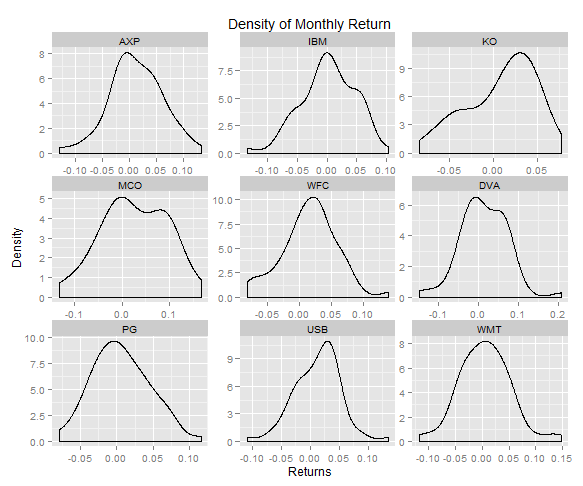
\includegraphics[width=.85\linewidth]{Density_of_Monthl_Return}
  	\centering
  	\caption{Density plots for all assets.}
\end{figure}

\begin{minipage}{\linewidth}
\begin{center}
\begin{tabular}{ |P{2cm}||P{2cm}|P{2cm}|P{2cm}|P{2cm}|P{2cm}|  }
 \hline
 \multicolumn{6}{|c|}{Univariate Fitting of Individual Assets} \\
 \hline
 Criteria  &  T-distribution & Skewed T-distribution & Generalized Error Distribution &  Skewed Generalized Error Distribution & Best Fit\\
 \hline
    AXP.AIC & -189.00 & -187.01 & -188.92 & -186.93 & t \\
    AXP.BIC & -182.67 & -178.57 & -182.59 & -178.49 & t \\
    IBM.AIC & -199.48 & -198.41 & -199.51 & -198.50 & ged \\
    IBM.BIC & -193.14 & -189.97 & -193.18 & -190.05 & ged \\
    KO.AIC & -216.27 & -223.46 & -220.26 & -223.47 & skewed ged \\
    KO.BIC & -209.94 & -215.02 & -213.93 & -215.02 & skewed ged \\
    MCO.AIC & -148.28 & -146.57 & -150.27 & -149.07 & ged \\
    MCO.BIC & -141.94 & -138.12 & -143.94 & -140.62 & ged \\
    WFC.AIC & -206.99 & -205.36 & -207.42 & -205.78 & ged \\
    WFC.BIC & -200.66 & -196.92 & -201.09 & -197.33 & ged \\
    DVA.AIC & -169.52 & -167.54 & -168.24 & -166.44 & t \\
    DVA.BIC & -163.19 & -159.09 & -161.90 & -158.00 & t \\
    PG.AIC & -216.48 & -215.88 & -216.54 & -215.91 & ged \\
    PG.BIC & -210.15 & -207.43 & -210.21 & -207.47 & ged \\
    USB.AIC & -216.51 & -216.61 & -215.43 & -216.27 & skewed t \\
    USB.BIC & -210.17 & -208.17 & -209.10 & -207.83 & t \\
    WMT.AIC & -194.74 & -192.95 & -194.26 & -192.54 & t \\
    WMT.BIC & -188.41 & -184.50 & -187.93 & -184.10 & t \\
 \hline
\end{tabular}
\bigskip \\
Table 13. Univatiate model fits.
\end{center}
\end{minipage}


\begin{thebibliography}{99}

\bibitem{c1} "Berkshire Hathaway Portfolio Tracker." CNBC. Web. 7 Dec. 2015. http://www.cnbc.com/berkshire-hathaway-portfolio/.

\bibitem{c2}"Selected Interest Rates (Daily) - H.15." FRB: H.15 Release--Selected Interest Rates--Historical Data. Web. 7 Dec. 2015. http://www.federalreserve.gov/releases/h15/data.htm.

\bibitem{c3} Ruppert, D. (2011). Statistics and data analysis for financial engineering. New York, NY: Springer.

\end{thebibliography}


\end{document} 